\section{Grasping novel objects based on familiar parts}
\label{cha3:sec4}
A method to compute grasps for novel objects is in need for domestic service robots. In this chapter we study the problem of generating grasps for un-trained objects in real time.

Objects used in daily life have a variety of shapes. Very often they share similar shape parts, such as sphere, cylinder and box. These shapes repeatedly appear in our daily life, being the object shape or the part of the object shape. Hence we call them``shape primitives''.

To work with un-trained objects, we take the grasping by shape primitives approach~\citep{miller2003automatic}. This approach makes the assumption that all object shapes can be decomposed into a set of primitive shapes where grasps can be planned easily. Based on this assumption, we firstly build a set of GMMs to model the grasp distribution $\left(\Omega_i, i=1,2,...N\right)$ for a set of $N$ chosen shape primitives. When an unseen object is presented, of which the shape can be approximated as a combination of known shape primitives, it's grasp distribution is built by combining the primitives' models. The combined model is then used to quickly generate new grasps.

%\subsection{Combine grasp distribution of shape primitives}
%\label{cha3:sec4:combine}


\subsection{Primitive grasp distribution}
\label{cha3:sec4:pgdistribution}
%\subsubsection{Primitive grasp distribution}
%\label{cha3:sec4:combine:primitivegraspdistribution}
Here we define our shape primitives to be a set of superquadrics. We learn the grasp distributions for a set of superquadrics and use them as the ``primitive grasp distribution''.


\paragraph{Superquadrics} ~\\
%\label{cha3:sec4:combine:primitivegraspdistribution:sq}
Superquadrics are a family of geometric shapes that includes a large variety of shapes we use in daily life, such as cuboid, sphere and cylinder. We choose superquadrics as our shape primitives for three reasons. Firstly, superquadrics and their combinations can be used to represent most of the daily life objects. The wide use of superquadrics in computer graphics and the game industry for modelling object shapes shows its versatility. Secondly, all superquadrics are symmetric to their $x, y, z$ axis. This can reduce the number of testing grasps to 1/8. Thirdly, it's implicit expression is convenient for combining the grasp density, which will be explained in detail in the Section~\ref{cha3:sec4:combine:combining}.

To represent a superquadric we have:

\begin{equation}
r\left(x, y ,z\right) =
\left(\left(\frac{x-x_0}{a_1}\right)^{\frac{2}{\epsilon_2}} +
    \left(\frac{y-y_0}{a_2}\right)^{\frac{2}{\epsilon_2}}\right)^
    {\frac{\epsilon_2}{\epsilon_1}} +
    \left(\frac{z-z_0}{a_3}\right)^\frac{2}{\epsilon_1}
\end{equation}
where $\left(x_0, y_0, z_0\right)$ is the center, $a_1, a_2, a_3$ define the scale in the $x, y, z$ axis respectively, and $\epsilon_1, \epsilon_2$ define the shape of the superquadric.
We use the value of $r$ to measure the relative position of a point $x, y, z$ to the superquadric shape:
\begin{equation}
    r
    \begin{cases}
      <1, & \text{inside the superquadric}\  \\
      =1, & \text{on the surface of the superquadric}\ \\
      >1, & \text{outside the superquadric}
    \end{cases}
\end{equation}

For sphere, cylinder and box primitives, the shape parameters are:

\begin{enumerate}
\item Sphere: $\epsilon_1 = 1, \epsilon_2 = 1$
\item Cylinder: $\epsilon_1 = 1, \epsilon_2 = 0.1$
\item Box: $\epsilon_1 = 0.1, \epsilon_2 = 0.1$
\end{enumerate}

Figure~\ref{fig:sq}~ shows how does the shape varies by these two factors~\footnote{Figure from internet source http://www.vincent-morio.com/content/en/gallery.html}.

\begin{figure}
  \centering
  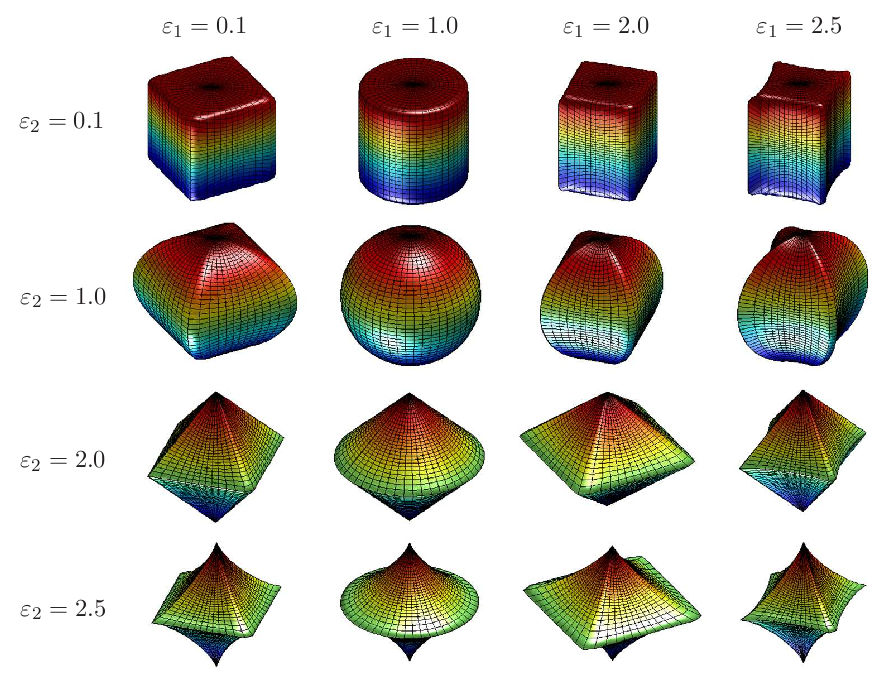
\includegraphics[width=14cm]{./fig_cha3/superquadrics.jpg}
  \caption{Illustration of 3D superquadric shapes with varying rounding parameters\protect\footnotemark.}
  \label{fig:sq}
\end{figure}


\paragraph{Learning grasp distributions for shape primitives}
%\label{cha3:sec4:combine:primitivegraspdistribution:learning}
~\\

With the method described in Section~\ref{cha3:sec2}, we build GMMs for the feasible grasp distributions for a set of shape primitives, i.e. superquadrics. Again, we model the distribution with a GMM as a sum of $K$ Gaussian components:

\begin{equation}
{
P (\boldsymbol{h},\boldsymbol{o},\boldsymbol\theta \text{\textbar} \varOmega)
= \sum_{k=1}^K {p_{k}p(\boldsymbol{h},\boldsymbol{o},\boldsymbol{\theta} \text{\textbar} {\boldsymbol{\mu}_k}, {\boldsymbol{\Sigma}_k})}
}
\end{equation}
where $k$ is the number of Gaussian components, $p_k$ the prior of the Gaussian component and the $\boldsymbol{\mu}_k$, $\boldsymbol{\Sigma}_k$ the corresponding mean and covariance.

Figure~\ref{fig:primtivedistr} visualizes the grasp distributions encoded by GMMs for three shape primitives: a box, a sphere and a cylinder. The robot hand we use here is the Barrett hand.

\begin{figure}
  \centering
    \subfloat[\scriptsize{Box}] {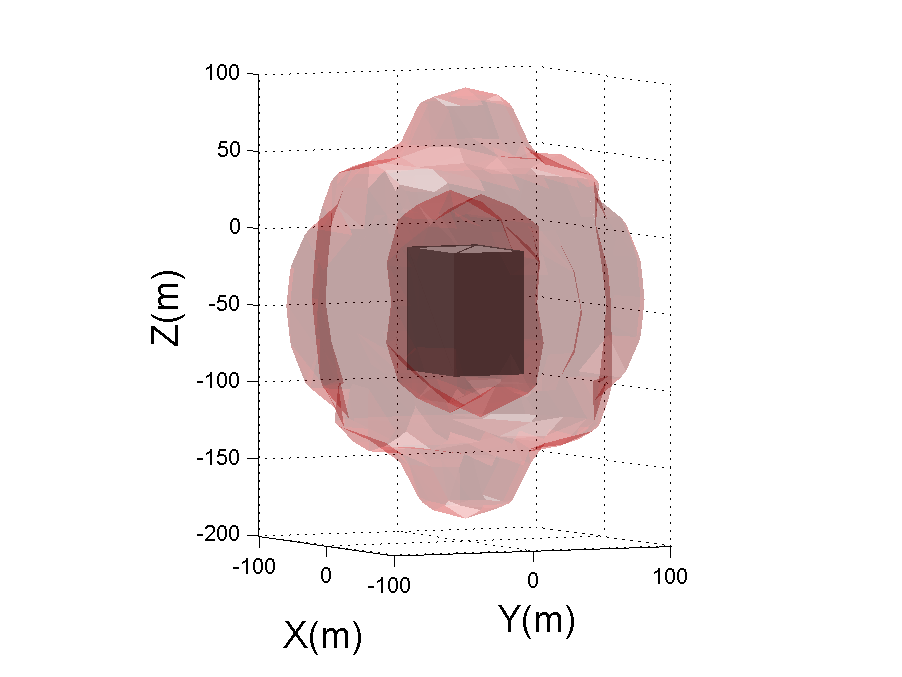
\includegraphics[width=4.5cm]{./fig_cha3/box1.eps}}
    \subfloat[\scriptsize{Sphere}]  {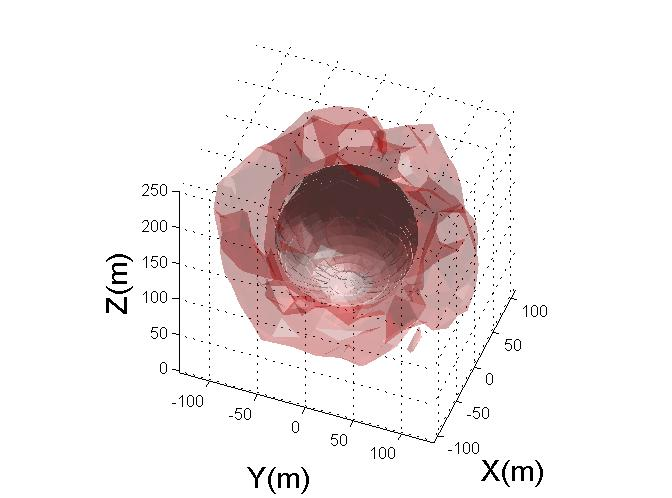
\includegraphics[width=4.5cm]{./fig_cha3/ball2.jpg}}
    \subfloat[\scriptsize{Cylinder}]  {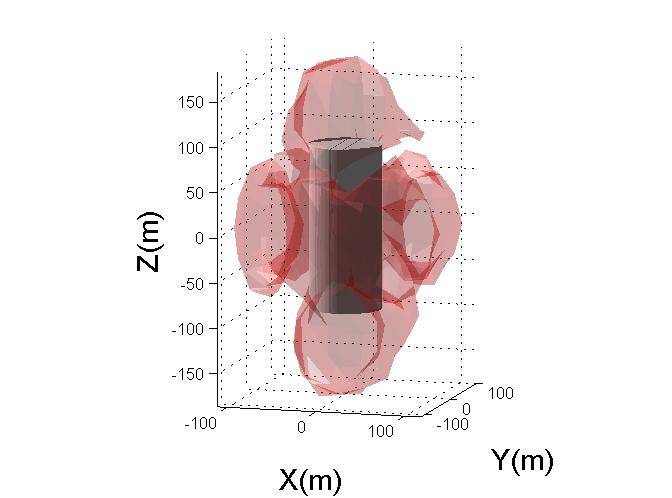
\includegraphics[width=4.5cm]{./fig_cha3/cyl.jpg}}
  \caption{A 3D visualization of the feasible grasp distribution for three shape primitives and the Barrett hand. The red contours are the isosurfaces of the grasp distribution. The ``redder'' the area is, the denser the distribution is.}
  \label{fig:primtivedistr}
\end{figure}


\subsubsection{Combining grasp distribution} ~\\
\label{cha3:sec4:combine:combining}
For an object composed of a few shape primitives, its grasp distribution is the combination of the the grasp distributions of its primitive components. However, this ``combination'' is not a summation of the GMMs: we need to exclude the grasps causing collision.

Before combining the grasp distributions, which are encoded by GMMs, of different shape primitive components of an object, we need to reshape each GMM by the object geometry. This is because when primitives combine to a more complex shape object, the grasp space of one part might be blocked by other part of the object.

For example, an object combined by a cylinder and a sphere is shown in Fig.~\ref{fig:object}(a) and it's primitives with their grasp distributions are shown in (b) and (c). As can be seen in (b) and (c), the top part of the grasp distribution of the cylinder will be inside the sphere and the bottom part of the grasp distribution of the sphere will be inside the cylinder. Grasps generated from these parts will cause collisions between the hand and the object and hence they have to be excluded from the model. 
% Finger collision
%Further, even when the robot hand is placed in a feasible location for all components, when the fingers clutch to grasp one component of the object, the moving trajectory of the finger might be blocked by other components. These kind of grasps should also be excluded from the grasp density of the whole object.
%Therefore, we take into account two kinds of collisions: collisions between the palm and the object and collisions between the finger trajectories and the object. 
To avoid collisions, we use the ``object sigmoid'' function to remove the collision parts.

\paragraph{Object sigmoid} ~\\
\label{cha3:sec4:combine:sigmoid}
We define a shape descriptor ``object sigmoid'' for objects modelled by a superquadric. The object sigmoid is a 3 dimensional sigmoid function defined as:
\begin{equation}
s\left(x, y ,z\right) = \frac{1}{1+e^{-100\left(r\left(x, y ,z\right)-1\right)}}
\label{equ:objectsigmoid}
\end{equation}
where r$\left(x, y ,z\right)$ is a function of the location defined in the form of a superquadrics. When we model an object shape with a superquadric, the object sigmoid has different values inside, on and outside the object:
\begin{equation}
    s
    \begin{cases}
        \rightarrow0, & \text{inside the object}\  \\
        =0.5 & \text{on the surface of the object}\ \\
        \rightarrow1 & \text{outside the object}
    \end{cases}
\end{equation}
In equation~\ref{equ:objectsigmoid} we choose a large coefficient, i.e. 100, for $r$ to make a sharp transition between 0 and 1 and hence a sharp cut on the object surface. Hence the object sigmoid gives a description of the shape of the object in the space: zero inside the object and one outside the object.

Each primitive component has its own object sigmoid. Before combining the individual distributions to form the whole distribution, each individual distribution is multiplied by all other components' object sigmoids. In this way, the likelihood inside the other parts of the object is reduced to zero, while the likelihood outside the object remains. The grasp distribution is hence ``trimmed'' by the other components of the object. The grasp distribution of the whole object is the summation of all the trimmed grasp distributions:

\begin{equation}
\boldsymbol{\Omega}\left(x,y,z\right) = \sum_{i=1,2..}^{N}\left(\Omega_i\prod_{j=1,2..\left(j\neq{i}\right)}^{N}s_j\right)
\end{equation}
where $\Omega_i$, $s_j$, $N$ is the grasp distribution of the $i-th$ primitive component, the object sigmoid of the $j-th$ primitive component and the total number of primitive components. The total number of Gaussians in the GMM of the whole object is the sum of the number of each primitives.

Figure.~\ref{fig:object}(d) shows the resulting grasp distribution of the whole object, which is the combination of the trimmed grasp GMM of the cylinder (Figure.~\ref{fig:object}(d)) and the sphere (Figure.~\ref{fig:object}(f)). Strictly speaking, the combined grasp distribution is not a density function, as the integral of the probability of the whole space is not normalized to one. Despite this, it does not effect the computation of a new grasp as we consider each Gaussian component individually.

\begin{figure}
\centering
    \hspace{-1cm}
    \begin{minipage}[c]{1\textwidth}
    \subfloat[\scriptsize{Novel object}]  {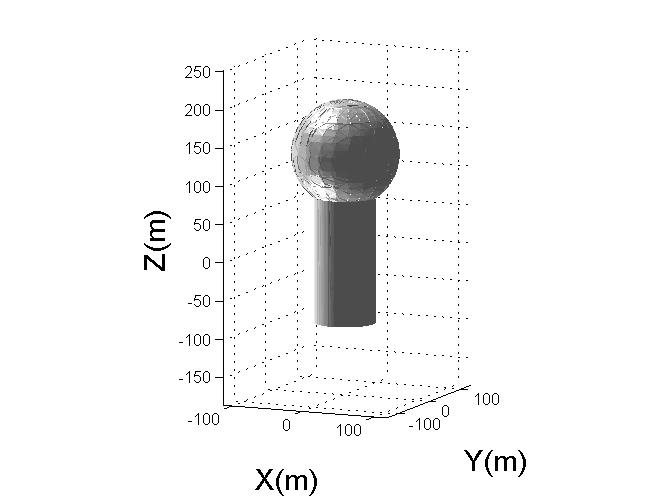
\includegraphics[width=5cm]{./fig_cha3/object.jpg}}
    \subfloat[\scriptsize{Cylinder grasp distribution}] {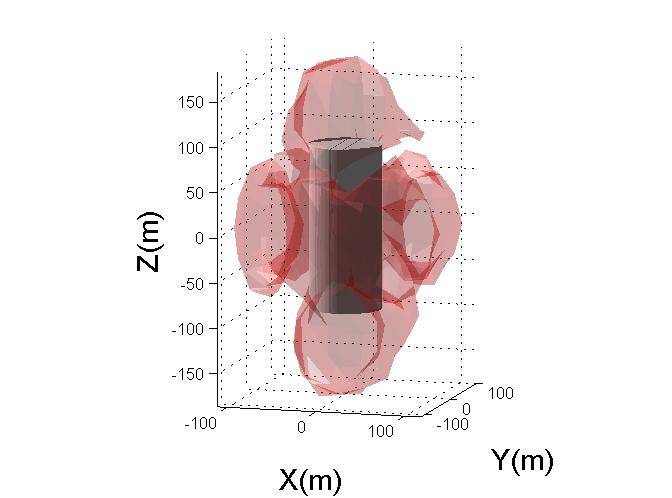
\includegraphics[width=5cm]{./fig_cha3/cyl.jpg}}
    \subfloat[\scriptsize{Sphere grasp distribution}] {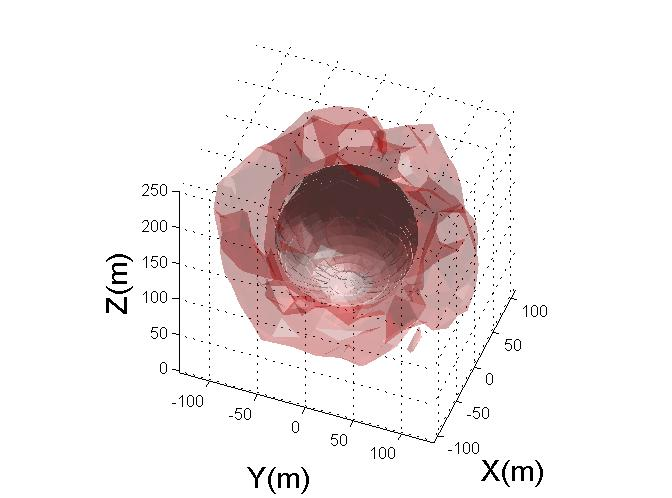
\includegraphics[width=5cm]{./fig_cha3/ball2.jpg}}



    \subfloat[\scriptsize{Combined object grasp distribution}] {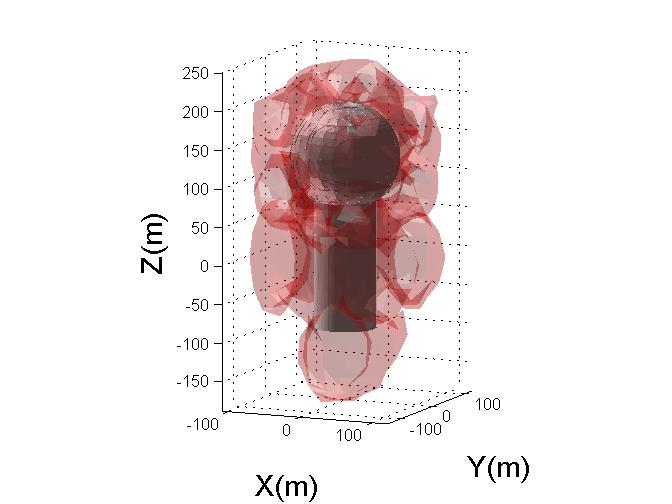
\includegraphics[width=5cm]{./fig_cha3/cylball.jpg}}
    \subfloat[\scriptsize{Trimmed grasp distribution}] {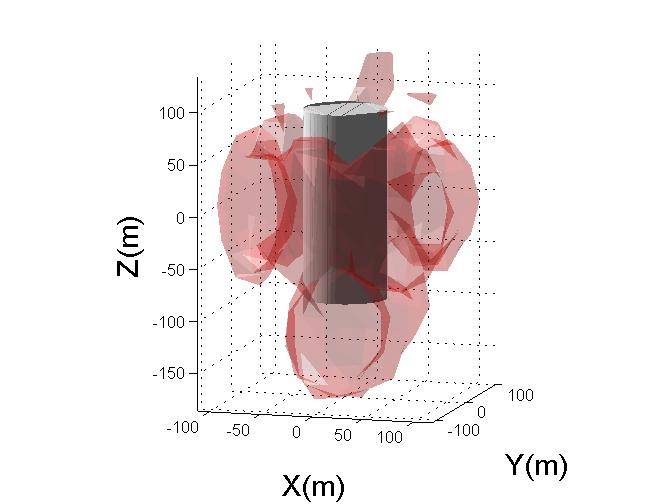
\includegraphics[width=5cm]{./fig_cha3/cyl_sig.jpg}}
    \subfloat[\scriptsize{Trimmed grasp distribution}] {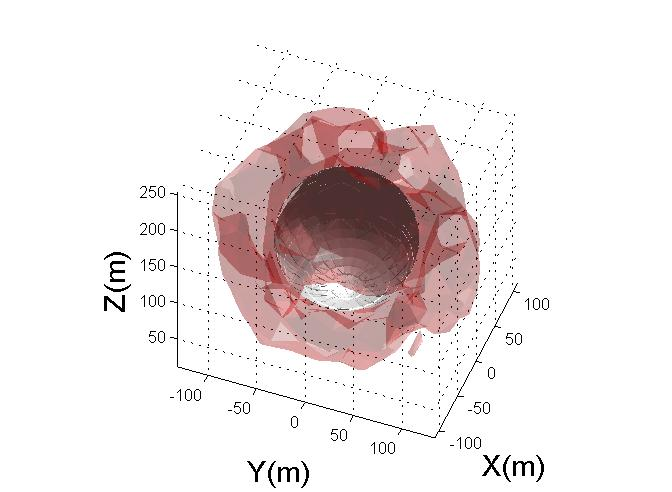
\includegraphics[width=5cm]{./fig_cha3/ball_sig2.jpg}}
    \end{minipage}

\caption{\scriptsize{(a) A combination of a cylinder and a sphere. (b) A 3D illustration of the grasp GMM of the cylinder. The red patch is the isosurface of the grasp GMM. (c) The grasp GMM of the sphere. (d) The combined grasp GMM of the whole object (d={e,f})). (e) The trimmed grasp GMM of the cylinder. The top part of the GMM is removed. (f) The trimmed grasp GMM of the sphere. Part of the bottom of the GMM is removed.}}
\label{fig:object}
\end{figure}


The equation above removes the grasps inside the object and hence avoids the collision between the robot palm and the object. 

% Finger collision
%However, grasps causing collision between finger trajectory and the object still remain.
%\paragraph{TODO: Trim grasp distribution by finger trajectory} ~\\


\subsection{Plan Grasp by combined grasp distribution}
\label{cha3:sec4:plan}

With the combined grasp distribution for the whole object, we can fast plan a grasp with the method described in Section~\ref{cha3:sec2}. Starting from an initial hand position and orientation $q = \{h, o\}$, the first step to compute a new grasp is to project $q$ to the feasible region of the GMM, where the probability of finding a stable grasp is high. This is done by finding the minimum Mahalanobis distance between $q$ and its projection point $q_k^\star$ in each Gaussian component of the GMM.

The projection point $q_k^{\star}$ of the $k$-th Gaussian component is computed as:
\begin{equation} \label{alpha}
q_k^{\star} = q + \alpha_k\left(q-\mu_k\right)
\end{equation}
where $\mu_k$ is the mean of the $k$-th Gaussian and $\alpha_k$ is a scalar determined by the boundary of the feasible region.

For $q_k^{\star}$ we have
\begin{equation} \label{qstar}
-\frac{1}{2}\left(q_k^{\star}-\mu_k\right)^T\Sigma_k^{-1}\left(q_k^\star-\mu_k\right)=-\frac{1}{2}\cdot{1}^{2}
\end{equation}
with equation~\ref{alpha} and~\ref{qstar}, $\alpha_k$ can be computed and hence $q_k^{\star}$.

The feasibility of each projection point is checked by the object sigmoids:

\begin{equation}
l_k = \prod_{j=1,2,...\left(j\neq{k}\right)}^N{s_j}
\end{equation}
If $l_k$ is smaller than 1, indicating that this point is inside or on the surface of the object, the likelihood at point $q^{\star}_k$ is zero.

We find the nearest projection point from the $q_k^\star$ with non-zero density. The nearest $q_k^\star$ is chosen to be the final grasp hand position and orientation $q^\star$. The grasp distribution $\Omega^{\star}$ which $q^{\star}$ locates in is used to compute the corresponding joint configuration though GMR. This allows us to compute the expected value of the finger joints from the conditional $p\left(\theta\mid{q^{\star}},\Omega^{\star}\right)$ (Section~\ref{cha3:sec2}). 